
\section{Precision-savvy algorithms: Aggregation v.s. Retrieval Comparison}
\begin{figure}[ht!]
   \centering%, trim=2cm 5cm 1cm 5cm]
   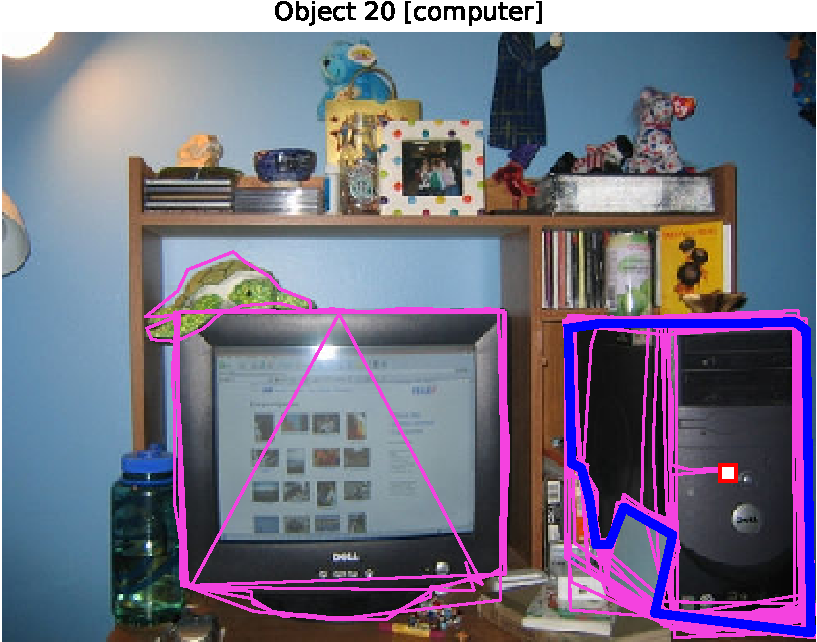
\includegraphics[width=.31\textwidth]{plots/bb_object_20.pdf}
   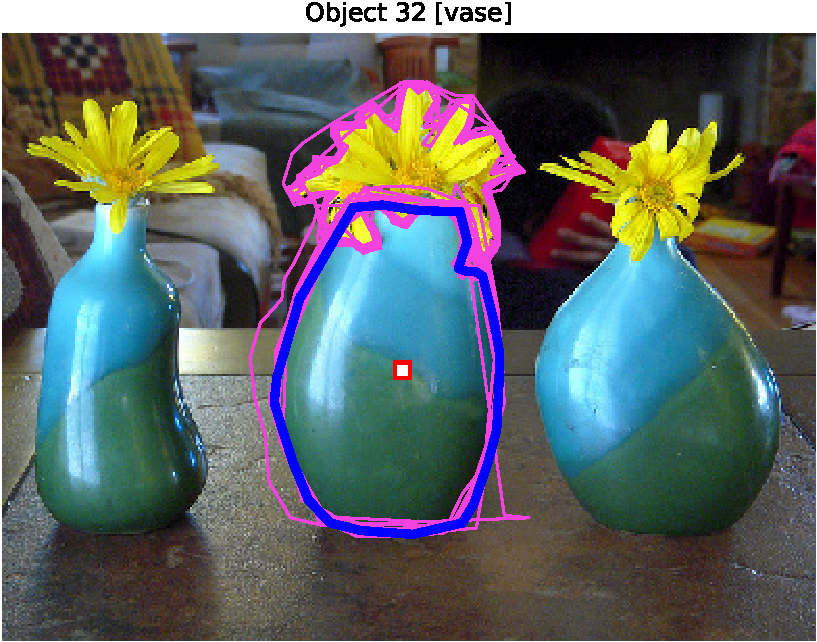
\includegraphics[width=.31\textwidth]{plots/bb_object_32.pdf}
   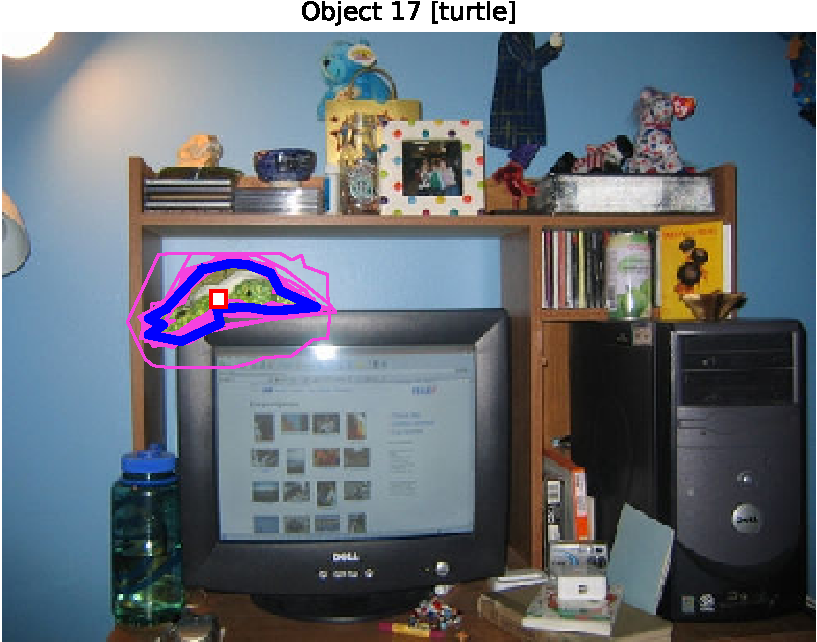
\includegraphics[width=.31\textwidth]{plots/bb_object_17.pdf}
   \caption{Pink is the segmentation from individual workers. Blue solid line delineates the ground truth. The red boxed pointer indicates the task of interest shown to users. Examples demonstrating common error patterns among crowdsourced image segmentation, including 1) annotations on the wrong semantic object, 2) ambiguity in regional inclusion and exclusion, and 3) imprecision at the object boundary.}
   \label{error_examples}
\end{figure}
\par As shown in Figure \ref{error_examples}, common worker errors can be classified into three types: (1) \textbf{Boundary Imprecision:} unintentional mistakes while drawing the boundaries, either due to low precision of the image, small area of the object, or lack of drawing skills , (2) \textbf{Semantic Ambiguity:} have differing opinions about whether particular regions belong to part of an object; or (3) \textbf{Semantic Mistakes:} annotate the wrong object entirely.
\par Out of the 46 objects in our dataset, 9 objects suffer from semantic ambiguity, 18 objects from semantic mistakes, and almost all objects suffer from some form of boundary imprecision to varying degrees. Since the main focus for quality evaluation in past literature have been focused on finding worker segmentation with minimal boundary precision issues, we will first describe novel aggregation-based algorithms that we have developed and compare them with existing retrieval-based methods for addressing type three errors. In the following section, we will discuss a preprocessing method that we have developed to resolve the semantic ambiguity and mistakes, which have been observed in prior work~\cite{Sorokin2008,Lin2014,Gurari2018}.
\subsection{Retrieval-based methods}
This class of algorithms tries to identify good and bad workers, and then chooses the best worker segmentation as the output segmentation. In this paper, we look at two different ways of ranking workers and choosing the best worker. First, we use the {\em number of control points}, i.e. number of vertices in a worker's segmentation polygon to rank workers. This is a ranking scheme that~\cite{Vittayakorn2011} showed performs well in practice. Intuitively, workers that have used a larger number of points are likely to have been more precise, and provided a more complex and accurate segmentation. Other heuristic ranking scheme is described in more detail in our technical report~\cite{segmentation-tr}.
\begin{figure}
\centering
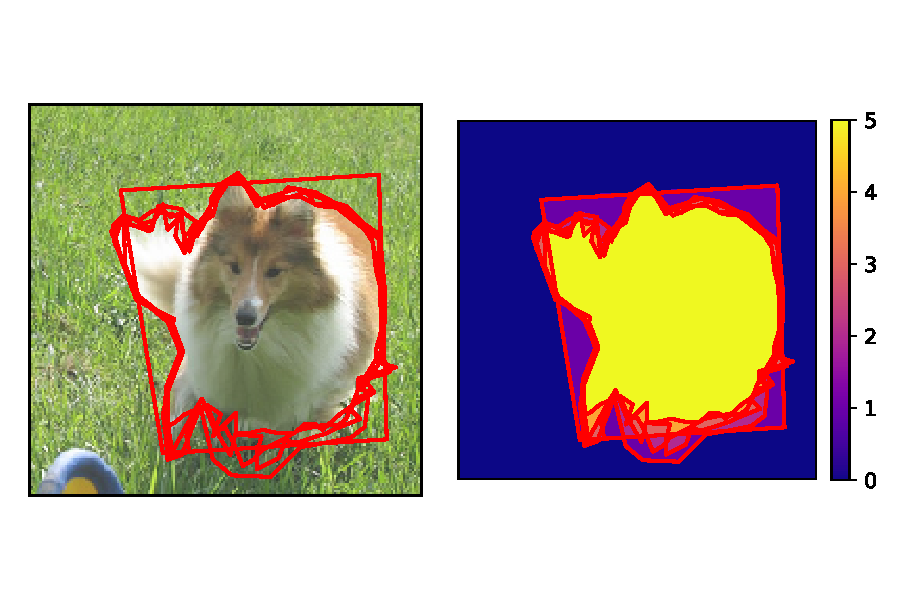
\includegraphics[width=\textwidth]{plots/tile_demo.pdf}
\caption{Left: Red boundaries shows the segmentation boundaries drawn by five workers overlaid on the image. Right: Segmentation boundaries still shown in red. The overlaid segmentation creates a masks where the color indicates the number of workers who voted for the tile region.}
\label{tile_demo}
\end{figure}
\subsection{Aggregation-based methods}
Rather than simply identifying and picking a single worker's segmentation, aggregation-based methods seek to combine multiple workers' segmentations into a single merged segmentation. At the heart of all our aggregation techniques is the following data representation: we logically overlay all workers' segmentations on top of each other within the framework of the overall image. As illustrated in \ref{tile_demo}, the overlaid worker segmentations can be thought of as a Venn diagram that represents a partitioning of the entire image into multiple worker {\em tiles} formed by the intersections of different worker segmentations. We then choose and merge a subset of the tiles to give the final output segmentation\dor{vague}. The intuition here is that by splitting the image into tiles, we get finer granularity information than by looking at complete segmentations. This also allows us to aggregate data from multiple workers rather than having to choose a single worker bounding box---this allows for the potential of choosing the best partial segmentations for an object and joining them, or fixing one worker's errors by taking the help of another worker's segmentation. The problem of choosing a good set of tiles is, however, non-trivial.
Since aggregation based methods are the least studied methods by previous work, we discuss them in further detail in Section~\ref{sec:agg-detailed}.


\subsection{Majority Vote Aggregation (MV)}
The aggregation-based majority vote algorithm examines --- tile, and includes the tile in the output segmentation if and only if the tile is covered by at least 50\% of all worker segmentations.
% We investigated three types of variants for majority vote strategies: picking the top-k, top-percentile tiles of vote counts and picking the tiles that were voted by at least 50\% of the workers. We found that among these majority vote variants, the latter strategy gave the highest accuracy.

\subsection{Expectation-Maximization}
While Majority Vote is a very useful algorithm in practice, it does not distinguish between workers in any way. In reality, however, not all workers are equal. Now, we try to model worker quality, and use worker quality information to infer the likelihood that a tile is part of the ground truth segmentation. Since both, the worker qualities, as well as the likelihoods of tiles being part of the ground truth are hidden quantities, we employ an Expectation-Maximization based approach to simultaneously esimtate both of these sets of quantities. We intuitively describe three worker models that we experiment with below. In our technical report, we formalize the notion of the probability that a set of tiles forms the ground truth, and solve the corresponding maximum likelihood problem, for each of these worker models.

\subheading{Worker quality models.}
We can think of workers as agents that look at each pixel in an image and label it as part of the segmentation, or not. Their actual segmentation is the union of all the pixels that they labeled as being part of their segmentations. Each pixel in the image is also either included in the ground truth segmentation or not included in the ground truth segmentation. We can now model worker segmentation as a set of boolean pixel-level (include or don't include) tasks, each having a ground truth boolean value. Based on this idea, we explore three worker quality models:
\begin{itemize}
\item {\em Basic model:} Each worker is captured by a single parameter Bernoulli model, $<q>$, which represents the probability that a worker will label an arbitrary pixel correctly.
\item {\em Ground truth inclusion model (GT):} Two parameter Bernoulli model $<qp, qn>$, capturing false positive and false negative rates of a worker. This helps to separate between workers that tend to overbound and workers that tend to underbound segmentations.
\item {\em Ground truth inclusion, large small area model (GTLSA):} Four parameter model $<qp_l, qn_l, qp_s, qn_s>$, that distinguishes between false positive and false negative rates for large and small tiles. In addition to capturing overbounding and underbounding tendencies, this model captures the fact that workers tend to make more mistakes on small tiles, and penalizes mistakes on large tiles more heavily.
\end{itemize}


\subsection{Greedy Tile Picking}\dor{the terminology ``overlap'' can be a bit confusing with the abbrev that we chose, since overlap area would be OA (rather than outside area). Maybe introduce it as intersection area or introduce terms ``inside'' and ``outside'' to correspond with the abbrev OA,IA.}
Next, we present a greedy tile picking algorithm that grows the output set of tiles by adding in one tile at a time. Suppose tile $t$, overlaps with the ground truth segmentation with intersection area of $IA(t)$, and has area $OA(t)$ not overlapping with the ground truth. The greedy algorithm sorts tiles in decreasing order of their $\frac{IA(t)}{OA(t)}$ ratio and iteratively adds the next tile to the growing set of output tiles, until the Jaccard value of the current set of tiles will decrease with the next added tile. \dor{explain intuition of why I/O is used.} The key idea behind this algorithm is the following statement\papertext{\todo[inline]{techreport}(proof available in our technical report)}: It can be shown that given a set of tiles, $T$, the tile $t$ that maximizes Jaccard($T\cup t$) score of the union of the set of tiles against the ground truth, is the tile with maximum value of $\frac{IA(t)}{OA(t)}$. The primary challenge with this approach is that we do not know the actual $IA(t)$, $OA(t)$ values for any tile. We implement a heuristic version of this algorithm, where we estimate the intersection area of any tile, $IA(t)$, by using the fraction of workers that have voted for a tile, and greedily maximize for estimated Jaccard value at every step. \papertext{\todo[inline]{techreport}In our technical report, we also discuss variants of this algorithm where we use different techniques to estimate the intersection areas of tiles, resulting in corresponding variants of the greedy algorithm.}
\subsection{What is the difference in performance between retrieval and aggregation-based methods?}
    Figure~\ref{retreival_vs_aggregation} shows the comparisons between the best performing algorithm amongst aggregation-based (greedy, EM) and retrieval-based (num points) algorithms. The solid line in Figure~\ref{retreival_vs_aggregation} shows algorithms that does not make use of ground truth information as part of the inference, while the dotted line shows the corresponding algorithm that makes use of ground truth information. Amongst the algorithms that do not make use of ground truth information, the performance of the greedy and EM algorithms exceeds the best achievable through existing retrieval-based method via the \texttt{num points} scoring heuristic and the vision-based algorithms. 
    \par By examining the dotted ground-truth algorithms, we learn the best achievable aggregation-based algorithm performs far better than the best worker segmentation. This result demonstrates since aggregation-based methods performs inference at a finer \textit{tile} granularity, it is able to achieve better performance than compared to retrieval-methods.
    \begin{figure}[h!]
      \centering
      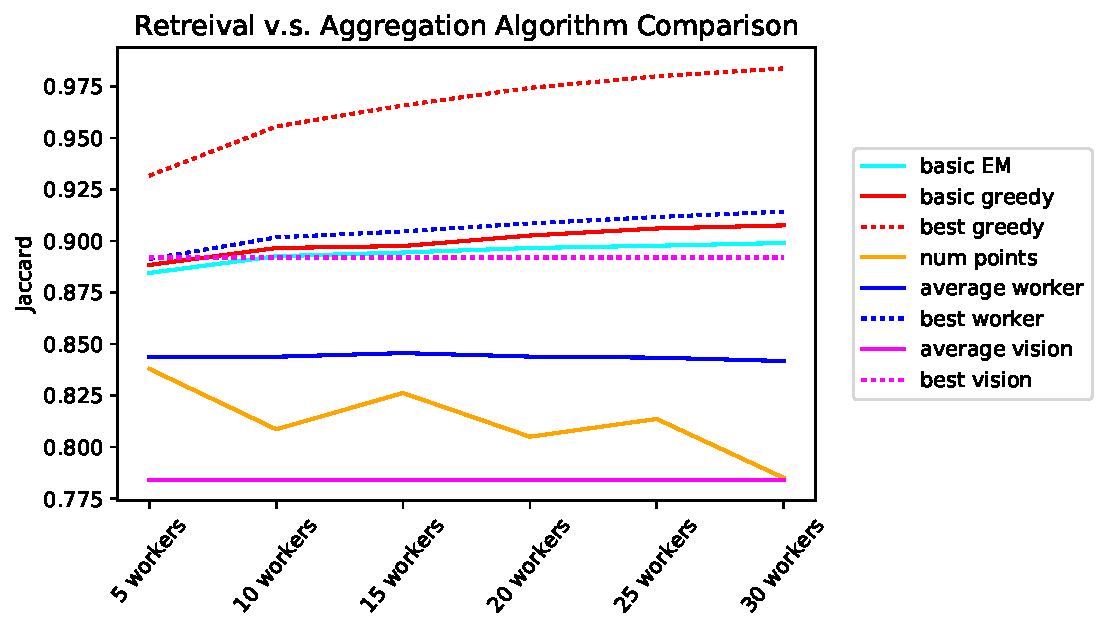
\includegraphics[width=\textwidth]{plots/Retreival_vs_Aggregation.pdf}
      \caption{Jaccard performance comparison between best-performing algorithms from retrieval and aggregation-based methods, with clustering as a preprocessing step where possible. Color denotes the type of algorithm used.}
      \label{retreival_vs_aggregation}
    \end{figure}
    \dor{We should split w/ GT and no GT information into two plots side by side with same color scheme. Also consider merging greedy and EM into just one that says aggregation based method, and renaming num points as retrevial based methods.}
    \par Table~\ref{workerScaling} shows that the three retrieval-based methods on the left do not improve the resulting Jaccard significantly when more annotations are used, whereas the right four aggregation-based methods improves significantly from the 5 worker to 30 worker sample. Intuitively, the worker scaling of retrieval-based methods is not guaranteed \footnote{except in the case of picking the best worker, the more samples means higher probability that there would be a better segmentation}. On the other hand, since larger worker samples results in finer granularity tiles for the aggregation-based methods, there is an monotonically increasing relationship between number of worker segmentation used in the sample and performance due to the finer tiles set created by multiple segmentations.
      \begin{table}
      \small
        \setlength\tabcolsep{1.5pt}
        \begin{tabular}{l|l|l|llll}
\multicolumn{3}{l|}{Retrieval-based} & \multicolumn{4}{l}{Aggregation-based}                                                             \\ \hline
num pts  & avrg worker & best worker & \multicolumn{1}{l|}{MV}   & \multicolumn{1}{l|}{EM}   & \multicolumn{1}{l|}{greedy} & best greedy \\ \hline
-6.30    & -0.25       & 2.58        & \multicolumn{1}{l|}{1.63} & \multicolumn{1}{l|}{1.64} & \multicolumn{1}{l|}{2.16}   & 5.59       
\end{tabular}
        \caption{Percentage change in Jaccard between 5 workers samples and 30 workers sample averages.}
        \label{workerScaling}
        \vspace{-10pt}
      \end{table}
      % as well as operating at a finer granularity that results in a higher potential upper bound.} 
      %Future work on developing better inference models would bring the performance closer to these upper bounds.
       \ta{Since aggregation-based methods operate at a finer tile-based granularity than whole-segmentation retrieval methods, the performance of aggregation-based approaches is better and also scales well as more annotations are collected.} 
       \par As shown in the dotted and solid line pairs in Figure~\ref{retreival_vs_aggregation}, when using ground truth to estimate intersection areas, we can achieve an average Jaccard of 0.983 as an upper bound with the 30 workers sample, which indicates that with better probabilistic estimation of intersection area, aggregation-based methods can achieve close to perfect segmentation outputs, exceeding the results than achievable by any single `best' worker (J=0.91 for 30 workers). Algorithms that gives users the option for collecting highly-accurate segmentation can have several useful applications in the biomedical domain~\cite{Gurari2015}.